% ============================================================
%  Lecture 1 — Course overview & Project Scheduling
% ============================================================

\section{Course Overview}
\label{sec:course-overview}

This course studies \emph{discrete optimisation problems}%
\aside{Discrete = integer-valued decisions: pick item 1, 2, 3\ldots{}
not a continuous value like 0.37.}
and, crucially, how to \emph{implement} algorithms that solve them.
Think of it as \emph{applied operations research}: we take the
mathematical models you have seen in Operations Research and turn
them into running code.

\medskip\noindent
The programme breaks into four blocks:

\begin{enumerate}[leftmargin=2em]
  \item \textbf{Problem survey} (Lectures 1--4).
    A tour of scheduling, timetabling, and logistics problems,
    together with the first solving technique: greedy algorithms.
  \item \textbf{Constraint modelling with MiniZinc.}
    We write a mathematical specification of the problem in the
    MiniZinc language; an underlying constraint-programming
    solver does the rest.
  \item \textbf{Advanced C++ and frameworks.}
    Inheritance, virtual functions, abstract classes, and the
    object-oriented framework we use for local search.
  \item \textbf{Solving techniques} (implemented in C++).
    Greedy, enumeration/backtracking, constraint programming
    (via MiniZinc), local search, and metaheuristics.
    Each technique is studied briefly in theory, then immediately
    applied to a concrete problem.
\end{enumerate}

\begin{remark}
  The exam is a \textbf{project}: choose a problem (proposed by
  the instructor or negotiated), solve it with at least two
  different techniques, and compare the results.
  Groups of at most two people; individual contributions
  are assessed during an oral discussion.
\end{remark}


% ============================================================
\section{Project Scheduling}
\label{sec:project-scheduling}
% ============================================================

Every project---building a house, developing a product, installing
a software stack---consists of activities with dependencies between
them.\aside{\texttt{apt install} internally solves
a project-scheduling instance over
package dependencies.}
The \emph{project scheduling problem} asks: given the activities
and their dependencies, when should each activity start so that the
whole project finishes as early as possible?

% ------------------------------------------------------------
\subsection{Problem definition}
\label{ssec:ps-definition}
% ------------------------------------------------------------

\begin{definition}[Project Scheduling Problem]
\label{def:project-scheduling}
We are given:
\begin{itemize}[nosep]
  \item a set of $n$ \emph{jobs} (activities) $\{1,\dots,n\}$,
        each with integer duration $d_i$;
  \item a set of \emph{precedence constraints}
        $P \subseteq \{1,\dots,n\}^2$,
        forming a \textbf{DAG} (directed acyclic graph):
        $(i,j)\in P$ means job~$j$ cannot start before job~$i$
        finishes.
\end{itemize}
We must assign a \emph{start time} $S_i\ge 0$ to every job
so that:
\begin{enumerate}[nosep]
  \item all precedences are respected:
        $S_j \ge S_i + d_i$ for every $(i,j)\in P$;
  \item the \emph{makespan} $\Cmax = \max_{i} (S_i + d_i)$
        is minimised.
\end{enumerate}
The completion time of job~$i$ is $C_i = S_i + d_i$.
\end{definition}

Let's unpack this.  We have a collection of jobs, each taking a
known amount of time.  Some jobs depend on others: job~$j$ can
only begin once every predecessor has finished.  The dependencies
form a directed acyclic graph---a DAG---because a cycle would make
the problem infeasible (if $A$ must precede~$B$ and $B$ must
precede~$A$, nothing can ever start).
Our goal is a single number: the makespan $\Cmax$, i.e.\ the
moment the \emph{last} job finishes.  We want it as small as
possible.

\begin{example}[Seven-job instance]
\label{ex:seven-jobs}
Consider seven jobs with the following durations and precedence
graph:

\begin{figure}[H]
\centering
\begin{tikzpicture}[
    job/.style={circle, draw=blue!60!black, fill=blue!8,
                minimum size=9mm, font=\small\bfseries},
    dur/.style={font=\footnotesize, text=gray!70!black},
    ->, >=Stealth, thick, node distance=18mm and 22mm
  ]
  % nodes
  \node[job] (1) {1};
  \node[job, above right=12mm and 22mm of 1] (2) {2};
  \node[job, below right=12mm and 22mm of 1] (3) {3};
  \node[job, right=22mm of 2] (4) {4};
  \node[job, right=22mm of 3] (5) {5};
  \node[job, above right=12mm and 22mm of 5] (6) {6};
  \node[job, above=8mm of 6] (7) {7};

  % durations (below each node)
  \node[dur, below=1mm of 1] {$d=3$};
  \node[dur, above=1mm of 2] {$d=3$};
  \node[dur, below=1mm of 3] {$d=1$};
  \node[dur, above=1mm of 4] {$d=4$};
  \node[dur, below=1mm of 5] {$d=2$};
  \node[dur, right=1mm of 6] {$d=1$};
  \node[dur, right=1mm of 7] {$d=3$};

  % arcs
  \draw (1) -- (2);
  \draw (1) -- (3);
  \draw (2) -- (4);
  \draw (3) -- (5);
  \draw (4) -- (6);
  \draw (5) -- (6);
  \draw (4) -- (7);
  \draw (5) -- (7);
\end{tikzpicture}
\caption{Precedence DAG for the seven-job instance
         (\cref{ex:seven-jobs}).
         Each node shows the job index; durations are labelled
         alongside.}
\label{fig:seven-job-dag}
\end{figure}

\noindent
Reading the graph: job~1 must finish before jobs~2 and~3 can
start; job~4 requires job~2; job~5 requires job~3; both jobs~6
and~7 require jobs~4 and~5.
\end{example}


% ------------------------------------------------------------
\subsection{What we leave out (for now)}
\label{ssec:ps-simplifications}
% ------------------------------------------------------------

The formulation above is deliberately simple.  Real-world projects
involve several complications that we set aside here but will
revisit in later lectures:

\begin{itemize}[nosep]
  \item \textbf{Resources.}
    Two independent jobs may still conflict if they both need the
    same machine or worker.
    Resource constraints turn the problem from polynomial to
    $\NP$-hard.
  \item \textbf{Release dates and deadlines.}
    A job may not be available before a certain date, or may have
    a hard deadline.
  \item \textbf{Uncertain durations.}
    In practice durations are stochastic (it might rain, a
    delivery might be late).
    One then minimises expected or worst-case makespan---this
    belongs to the Project Management course.
  \item \textbf{Generalised precedences.}
    Start-to-start, finish-to-finish, or time-lag constraints
    (e.g.\ concrete must be poured within a window after mixing).
  \item \textbf{Variable durations with costs.}
    Crashing: pay more to shorten a job.  This introduces a
    cost--time trade-off (multi-objective).
\end{itemize}


% ============================================================
\section{The Critical Path Method (CPM)}
\label{sec:cpm}
% ============================================================

The Critical Path Method is a classical greedy algorithm that
solves the basic project scheduling problem
(\cref{def:project-scheduling}) \emph{optimally}.%
\aside{Walker \& Kelley, late 1950s.
Originally for plant maintenance
shutdowns at DuPont.}

The idea is disarmingly simple: schedule every job as early as
possible, respecting precedences.  We formalise this in two
passes---forward and backward---and then combine them to identify
the \emph{critical path}.

% ------------------------------------------------------------
\subsection{CPM Forward (earliest schedule)}
\label{ssec:cpm-forward}
% ------------------------------------------------------------

\begin{definition}[CPM Forward]
\label{def:cpm-forward}
Process jobs in \emph{topological order} of the precedence DAG:
\begin{enumerate}[nosep]
  \item For every job~$i$ with no predecessors, set $S_i = 0$.
  \item For every other job~$i$ (once all predecessors are
        scheduled):
        \[
          S_i = \max_{(k,i)\in P}\; C_k
              = \max_{(k,i)\in P}\; (S_k + d_k).
        \]
  \item Set $C_i = S_i + d_i$.
\end{enumerate}
The makespan is $\Cmax = \max_{i=1}^{n} C_i$.
\end{definition}

In words: each job starts at the earliest moment all its
predecessors have finished.  We simply walk through the DAG
from sources to sinks, computing start and finish times as we go.

\begin{example}[CPM Forward on the seven-job instance]
\label{ex:cpm-forward}
Applying CPM Forward to \cref{ex:seven-jobs}:

\begin{figure}[H]
\centering
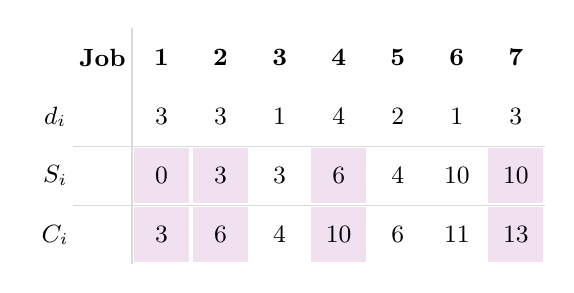
\begin{tikzpicture}[
    cell/.style={minimum width=7mm, minimum height=7mm,
                 font=\small, anchor=center},
    hdr/.style={cell, font=\small\bfseries},
    crit/.style={fill=violet!12},
    x=7.5mm, y=7.5mm
  ]
  % header row
  \foreach \j/\lbl in {1/Job, 2/1, 3/2, 4/3, 5/4, 6/5, 7/6, 8/7} {
    \node[hdr] at (\j, 4) {\lbl};
  }
  % d_i
  \node[cell, font=\small\itshape] at (0.2, 3) {$d_i$};
  \foreach \j/\v in {2/3, 3/3, 4/1, 5/4, 6/2, 7/1, 8/3} {
    \node[cell] at (\j, 3) {\v};
  }
  % S_i (forward)
  \node[cell, font=\small\itshape] at (0.2, 2) {$S_i$};
  \foreach \j/\v/\c in {2/0/crit, 3/3/crit, 4/3/, 5/6/crit, 6/4/, 7/10/, 8/10/crit} {
    \node[cell, \c] at (\j, 2) {\v};
  }
  % C_i (forward)
  \node[cell, font=\small\itshape] at (0.2, 1) {$C_i$};
  \foreach \j/\v/\c in {2/3/crit, 3/6/crit, 4/4/, 5/10/crit, 6/6/, 7/11/, 8/13/crit} {
    \node[cell, \c] at (\j, 1) {\v};
  }
  % grid lines
  \draw[gray!30] (1.5, 0.5) -- (1.5, 4.5);
  \draw[gray!30] (0.5, 2.5) -- (8.5, 2.5);
  \draw[gray!30] (0.5, 1.5) -- (8.5, 1.5);
\end{tikzpicture}
\caption{Earliest start and completion times (CPM Forward).
         \colorbox{violet!12}{Highlighted} cells belong to the
         critical path.}
\label{fig:cpm-forward-table}
\end{figure}

\noindent
Let's trace the computation step by step:
\begin{itemize}[nosep]
  \item Job~1 has no predecessors: $S_1 = 0$, $C_1 = 3$.
  \item Jobs~2, 3 depend only on job~1:
        $S_2 = C_1 = 3$, $C_2 = 6$; \;
        $S_3 = C_1 = 3$, $C_3 = 4$.
  \item Job~4 depends on job~2: $S_4 = C_2 = 6$, $C_4 = 10$.
  \item Job~5 depends on job~3: $S_5 = C_3 = 4$, $C_5 = 6$.
  \item Job~6 depends on jobs~4 and~5:
        $S_6 = \max(C_4, C_5) = \max(10, 6) = 10$, $C_6 = 11$.
  \item Job~7 depends on jobs~4 and~5:
        $S_7 = \max(C_4, C_5) = 10$, $C_7 = 13$.
\end{itemize}
The makespan is $\Cmax = \max(C_6, C_7) = 13$.
\end{example}

% ------------------------------------------------------------
\subsection{CPM Backward (latest schedule)}
\label{ssec:cpm-backward}
% ------------------------------------------------------------

The backward pass assumes we already know the makespan~$M$ from
the forward pass and asks: what is the \emph{latest} each job can
start without increasing $M$?

\begin{definition}[CPM Backward]
\label{def:cpm-backward}
Let $M = \Cmax$ from the forward pass.
Process jobs in \emph{reverse} topological order:
\begin{enumerate}[nosep]
  \item For every job~$i$ with no successors, set
        $C_i^{\,\text{late}} = M$.
  \item For every other job~$i$ (once all successors are
        scheduled):
        \[
          C_i^{\,\text{late}}
            = \min_{(i,j)\in P}\; S_j^{\,\text{late}}.
        \]
  \item Set $S_i^{\,\text{late}} = C_i^{\,\text{late}} - d_i$.
\end{enumerate}
\end{definition}

Notice the symmetry: forward uses $\max$ over predecessors;
backward uses $\min$ over successors.  The forward pass pushes
everything as early as possible; the backward pass pulls everything
as late as possible.

\begin{example}[CPM Backward on the seven-job instance]
\label{ex:cpm-backward}
With $M = 13$ from \cref{ex:cpm-forward}:

\begin{figure}[H]
\centering
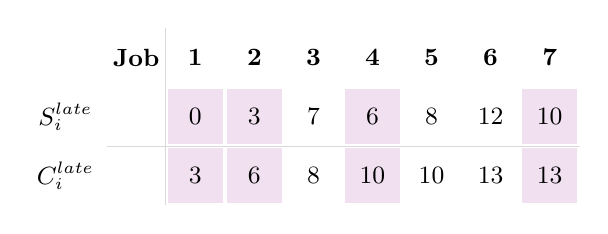
\begin{tikzpicture}[
    cell/.style={minimum width=7mm, minimum height=7mm,
                 font=\small, anchor=center},
    hdr/.style={cell, font=\small\bfseries},
    crit/.style={fill=violet!12},
    x=7.5mm, y=7.5mm
  ]
  % header
  \foreach \j/\lbl in {1/Job, 2/1, 3/2, 4/3, 5/4, 6/5, 7/6, 8/7} {
    \node[hdr] at (\j, 3) {\lbl};
  }
  % S_i^late
  \node[cell, font=\small\itshape] at (-0.2, 2) {$S_i^{\text{late}}$};
  \foreach \j/\v/\c in {2/0/crit, 3/3/crit, 4/7/, 5/6/crit, 6/8/, 7/12/, 8/10/crit} {
    \node[cell, \c] at (\j, 2) {\v};
  }
  % C_i^late
  \node[cell, font=\small\itshape] at (-0.2, 1) {$C_i^{\text{late}}$};
  \foreach \j/\v/\c in {2/3/crit, 3/6/crit, 4/8/, 5/10/crit, 6/10/, 7/13/, 8/13/crit} {
    \node[cell, \c] at (\j, 1) {\v};
  }
  % grid lines
  \draw[gray!30] (1.5, 0.5) -- (1.5, 3.5);
  \draw[gray!30] (0.5, 1.5) -- (8.5, 1.5);
\end{tikzpicture}
\caption{Latest start and completion times (CPM Backward).}
\label{fig:cpm-backward-table}
\end{figure}

\noindent
Tracing backwards from the sinks:
\begin{itemize}[nosep]
  \item Jobs~6 and~7 have no successors:
        $C_6^{\text{late}} = C_7^{\text{late}} = 13$.
        So $S_6^{\text{late}} = 12$, $S_7^{\text{late}} = 10$.
  \item Job~4: successors are 6 and 7.
        $C_4^{\text{late}} = \min(S_6^{\text{late}},
        S_7^{\text{late}}) = \min(12, 10) = 10$,
        $S_4^{\text{late}} = 6$.
  \item Job~5: successors are 6 and 7.
        $C_5^{\text{late}} = \min(12, 10) = 10$,
        $S_5^{\text{late}} = 8$.
  \item Job~2: successor is 4.
        $C_2^{\text{late}} = S_4^{\text{late}} = 6$,
        $S_2^{\text{late}} = 3$.
  \item Job~3: successor is 5.
        $C_3^{\text{late}} = S_5^{\text{late}} = 8$,
        $S_3^{\text{late}} = 7$.
  \item Job~1: successors are 2 and 3.
        $C_1^{\text{late}} = \min(3, 7) = 3$,
        $S_1^{\text{late}} = 0$.
\end{itemize}
\end{example}

% ------------------------------------------------------------
\subsection{The critical path}
\label{ssec:critical-path}
% ------------------------------------------------------------

\begin{definition}[Critical activity and critical path]
\label{def:critical-path}
A job~$i$ is \emph{critical} if its earliest and latest start
times coincide: $S_i = S_i^{\,\text{late}}$.
The \emph{critical path} is the set of all critical activities
(and the precedence arcs connecting them).
\end{definition}

A critical job has \emph{zero slack}: any delay in its execution
directly increases the makespan.  Non-critical jobs have
\emph{float}---they can shift within the interval
$[S_i,\; S_i^{\text{late}}]$ without affecting $\Cmax$.

\begin{example}[Critical path of the seven-job instance]
\label{ex:critical-path}
Comparing the forward and backward tables:

\medskip
\begin{center}
\begin{tabular}{lccccccc}
\toprule
\textbf{Job}             & 1 & 2 & 3 & 4 & 5 & 6 & 7 \\
\midrule
$S_i$ (earliest)         & 0 & 3 & 3 & 6 & 4 & 10 & 10 \\
$S_i^{\text{late}}$ (latest) & 0 & 3 & 7 & 6 & 8 & 12 & 10 \\
\midrule
Slack                    & 0 & 0 & 4 & 0 & 4 & 2  & 0 \\
Critical?                & \checkmark & \checkmark & & \checkmark & & & \checkmark \\
\bottomrule
\end{tabular}
\end{center}

\medskip\noindent
The critical path is $1 \to 2 \to 4 \to 7$, with
a total duration of $3 + 3 + 4 + 3 = 13 = \Cmax$.

\begin{figure}[H]
\centering
\begin{tikzpicture}[
    job/.style={circle, draw=blue!60!black, fill=blue!8,
                minimum size=9mm, font=\small\bfseries},
    cjob/.style={circle, draw=violet!70!black, fill=violet!15,
                 minimum size=9mm, font=\small\bfseries},
    dur/.style={font=\footnotesize, text=gray!70!black},
    ->, >=Stealth, thick, node distance=18mm and 22mm
  ]
  % critical nodes in violet
  \node[cjob] (1) {1};
  \node[cjob, above right=12mm and 22mm of 1] (2) {2};
  \node[job,  below right=12mm and 22mm of 1] (3) {3};
  \node[cjob, right=22mm of 2] (4) {4};
  \node[job,  right=22mm of 3] (5) {5};
  \node[job,  above right=12mm and 22mm of 5] (6) {6};
  \node[cjob, above=8mm of 6] (7) {7};

  % durations
  \node[dur, below=1mm of 1] {$d=3$};
  \node[dur, above=1mm of 2] {$d=3$};
  \node[dur, below=1mm of 3] {$d=1$};
  \node[dur, above=1mm of 4] {$d=4$};
  \node[dur, below=1mm of 5] {$d=2$};
  \node[dur, right=1mm of 6] {$d=1$};
  \node[dur, right=1mm of 7] {$d=3$};

  % critical arcs (violet, thicker)
  \draw[violet!70!black, line width=1.8pt] (1) -- (2);
  \draw[violet!70!black, line width=1.8pt] (2) -- (4);
  \draw[violet!70!black, line width=1.8pt] (4) -- (7);

  % non-critical arcs (gray)
  \draw[gray!50] (1) -- (3);
  \draw[gray!50] (3) -- (5);
  \draw[gray!50] (4) -- (6);
  \draw[gray!50] (5) -- (6);
  \draw[gray!50] (5) -- (7);
\end{tikzpicture}
\caption{The critical path $1 \to 2 \to 4 \to 7$
         (violet nodes and edges).
         Non-critical jobs and arcs are shown in gray.}
\label{fig:critical-path}
\end{figure}

\noindent
Job~3, for instance, can start anywhere between time~3 (earliest)
and time~7 (latest) without affecting the makespan.
Job~7, however, is locked: if it starts even one unit later, the
project finishes later.
\end{example}


% ------------------------------------------------------------
\subsection{Optimality of CPM}
\label{ssec:cpm-optimality}
% ------------------------------------------------------------

\begin{theorem}[CPM is optimal]
\label{thm:cpm-optimal}
The CPM Forward schedule achieves the minimum possible makespan
for the project scheduling problem
(\cref{def:project-scheduling}).
\end{theorem}

\begin{formaldetails}[Optimality of CPM]
The proof is by contradiction.
Consider the critical path $i_1 \to i_2 \to \cdots \to i_k$
found by CPM\@.
Every job on this path starts exactly when its predecessor
finishes (zero slack), so the makespan equals
\[
  \Cmax = d_{i_1} + d_{i_2} + \cdots + d_{i_k}.
\]
Any feasible schedule must respect the precedence chain
$i_1 \to i_2 \to \cdots \to i_k$, which means
\[
  \Cmax^* \;\ge\; d_{i_1} + d_{i_2} + \cdots + d_{i_k}
          \;=\; \Cmax.
\]
Since CPM produces a feasible schedule with makespan $\Cmax$,
and no feasible schedule can do better, CPM is optimal.
\qed
\end{formaldetails}

The key insight is that the critical path acts as a
\emph{lower bound}: no matter how cleverly we rearrange jobs,
we can never avoid executing every job on the critical path
in sequence, so the makespan is at least the sum of their
durations.  CPM \emph{achieves} this bound, so it is optimal.


% ============================================================
\section{Greedy Algorithms}
\label{sec:greedy-intro}
% ============================================================

CPM is our first example of a \textbf{greedy algorithm}.%
\aside{Italian: \emph{algoritmo avido};
the English ``greedy'' is standard.}

\begin{definition}[Greedy algorithm (informal)]
\label{def:greedy}
A greedy algorithm builds a solution incrementally.  At each step
it makes the locally best choice (assign the earliest possible
start time, pick the shortest job, etc.)\ and \emph{never
reconsiders} that choice.
\end{definition}

Greedy algorithms are typically very fast---often polynomial
time---because they never backtrack.  The catch is that for many
problems the locally best choice is not globally optimal.
CPM is a happy exception: the greedy ``start as early as possible''
rule happens to be provably optimal for the basic project
scheduling problem.

\begin{observation}
For more complex scheduling problems (with resources, deadlines,
or variable durations), greedy algorithms generally do \emph{not}
find the optimal solution.  We will need more powerful techniques:
enumeration, constraint programming, and local search.
\end{observation}


% ============================================================
\section{Algorithmic Analysis: Two Key Questions}
\label{sec:algo-analysis}
% ============================================================

Whenever we study a new algorithm, we ask two questions:

\begin{enumerate}
  \item \textbf{Computational complexity.}
    How does the running time scale with the input size?
    CPM processes each job once and inspects each precedence arc
    once, so its complexity is
    $\Oh{n + |P|}$%
    \aside{$|P|$ = number of arcs.  Worst case
    $\Oh{n^2}$; in practice graphs are
    sparse, so nearly linear.}---linear in the size of the input.

  \item \textbf{Exactness.}
    Does the algorithm always find the optimal solution?
    As we proved in \cref{thm:cpm-optimal}, CPM is \emph{exact}
    for the basic project scheduling problem.
\end{enumerate}

\begin{intermezzo}{CPM at scale}
In the lecture demo, a C++ implementation of CPM solved an
instance with \textbf{one million jobs} in about 4~seconds, and
instances with over 10~million jobs in under a minute.
The algorithm's simplicity---a single topological-order pass
through the DAG---translates directly into practical speed.
This is the power of a well-chosen greedy algorithm on a problem
where greedy happens to be optimal.
\end{intermezzo}


% ============================================================
\section{Instance Format}
\label{sec:instance-format}
% ============================================================

For the project scheduling problem we use a simple text format:%
\aside{Richer formats for more complex
problems; this suffices for the basic case.}

\begin{lstlisting}[language={}, caption={Instance file format
  for project scheduling.}, label={lst:ps-format}]
n                          (* number of jobs *)
d_1  #pred_1  pred_1a pred_1b ...
d_2  #pred_2  pred_2a pred_2b ...
...
d_n  #pred_n  pred_na pred_nb ...
\end{lstlisting}

\noindent
The first line gives the number of jobs~$n$.
Each subsequent line~$i$ (for $i = 1, \dots, n$) contains:
the duration~$d_i$, the number of predecessors, and the list of
predecessor indices.

\begin{example}[Instance file for \cref{ex:seven-jobs}]
\label{ex:instance-file}
\begin{lstlisting}[language={}, numbers=none]
7
3  0
3  1  1
1  1  1
4  1  2
2  1  3
1  2  4  5
3  2  4  5
\end{lstlisting}
Job~1 (line~2) has duration~3 and no predecessors.
Job~6 (line~7) has duration~1 and two predecessors: jobs~4 and~5.
\end{example}
